\documentclass[12pt]{article}
\usepackage{amsmath, amsfonts, amssymb}
\usepackage{tikz-cd}

\begin{document}

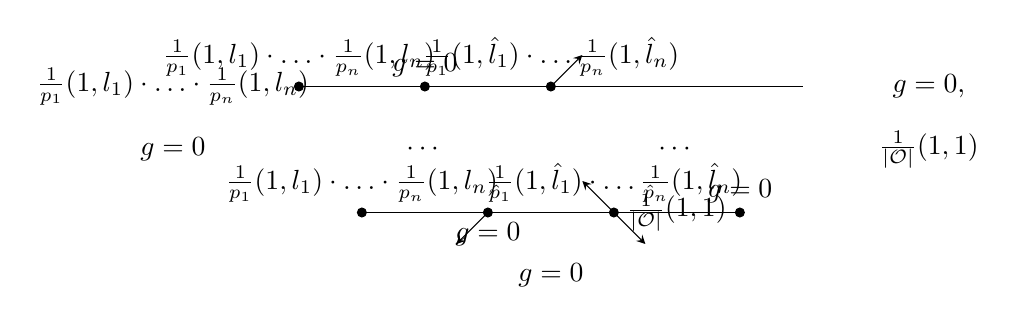
\begin{tikzpicture}[scale=0.8]
    % Define coordinates for the points
    \coordinate (A) at (-4, 1);
    \coordinate (B) at (-2, 1);
    \coordinate (C) at (0, 1);
    \coordinate (D) at (2, 1);
    \coordinate (E) at (4, 1);
    \coordinate (F) at (-3, -1);
    \coordinate (G) at (-1, -1);
    \coordinate (H) at (1, -1);
    \coordinate (I) at (3, -1);
    
    % Draw the lines connecting the points
    \draw (A) -- (B);
    \draw (B) -- (C);
    \draw (C) -- (D);
    \draw (D) -- (E);
    \draw (F) -- (G);
    \draw (G) -- (H);
    \draw (H) -- (I);
    
    % Draw the circles at the end points
    \filldraw [black] (A) circle (2pt) node[anchor=south] {$\frac{1}{p_{1}}(1,l_1)\cdot\ldots\cdot\frac{1}{p_{n}}(1,l_n)$};
    \filldraw [black] (B) circle (2pt) node[anchor=south] {$g=0$};
    \filldraw [black] (C) circle (2pt) node[anchor=south] {$\frac{1}{p_{1}}(1,\hat{l}_1)\cdot\ldots\frac{1}{p_{n}}(1,\hat{l}_n)$};
    
    \filldraw [black] (F) circle (2pt) node[anchor=south] {$\frac{1}{p_{1}}(1,l_1)\cdot\ldots\cdot\frac{1}{p_{n}}(1,l_n)$};
    \filldraw [black] (G) circle (2pt) node[anchor=north] {$g=0$};
    \filldraw [black] (H) circle (2pt) node[anchor=south] {$\frac{1}{\hat{p}_{1}}(1,\hat{l}_1)\cdot\ldots\frac{1}{\hat{p}_{n}}(1,\hat{l}_n)$};
    
    \filldraw [black] (I) circle (2pt) node[anchor=south] {$g=0$};
    
    % Arrows to indicate birational equivalence
    \draw[-stealth] (C) -- ++(0.5, 0.5);
    \draw[-stealth] (H) -- ++(-0.5, 0.5);
    \draw[-stealth] (H) -- ++(0.5, -0.5);
    \draw[-stealth] (G) -- ++(-0.5, -0.5);
    
    % Additional details
    \node at (-2, 0) {$\cdots$};
    \node at (0, -2) {$g=0$};
    \node at (2, 0) {$\cdots$};
    
    \node at (-6, 1) {$\frac{1}{p_{1}}(1,l_1)\cdot\ldots\cdot\frac{1}{p_{n}}(1,l_n)$};
    \node at (-6, 0) {$g=0$};
    
    \node at (6, 1) {$g=0$,};
    \node at (6, 0) {$\frac{1}{|\mathcal{O}|}(1,1)$};
    \node at (2, -1) {$\frac{1}{|\mathcal{O}|}(1,1)$};
    
\end{tikzpicture}

\textit{Birational equivalence of} $\mathbb{P}(L \oplus \mathbb{C})$ \textit{to a weighted projective plane, for an orbi-bundle} $L$ \textit{over an orbi-sphere.}